\documentclass{beamer}
%\usetheme{}%\usecolortheme{}
\setbeamertemplate{navigation symbols}{}
\setbeamertemplate{section in toc}[sections numbered]
\setbeamertemplate{footline}[frame number]

\usepackage[utf8]{inputenc}
\usepackage[T1]{fontenc}
\usepackage{lmodern}
\usepackage{appendixnumberbeamer}
\usepackage{multirow}

\title{%
  \textbf{BEST: a Binary Executable Slicing Tool}
  \\ and its use to improve
  \\ Model Checking-based WCET Analysis}
\author{%
  \textbf{Armel Mangean}$^1$
  \and Jean-Luc Béchennec$^2$
  \and Mikaël Briday$^3$
  \and Sébastien Faucou$^3$}
\institute{%
  IRCCyN, UMR CNRS 6597
  \\ $^1$École Centrale de Nantes, $^2$CNRS , $^3$Université de Nantes}
\date{July 5, 2016}

% 20 min -> ~15 slides

\begin{document}

  \begin{frame}
    \titlepage

    \begin{center}
      
\includegraphics[height=0.8cm]{fig/irccyn.png}
    \end{center}

    \emph{\small 16th International Workshop on Worst-Case Execution Time Analysis}
  \end{frame}

  \begin{frame}
    \frametitle{~}
    \tableofcontents
  \end{frame}

  %%%
  
  \section{Introduction}
  \begin{frame}
    \frametitle{\secname}
    \tableofcontents[currentsection]
  \end{frame}
  
  \subsection{Motivation}
  \begin{frame}
    \frametitle{\secname}
    \framesubtitle{\subsecname}
    
    \begin{figure}
      \centering
      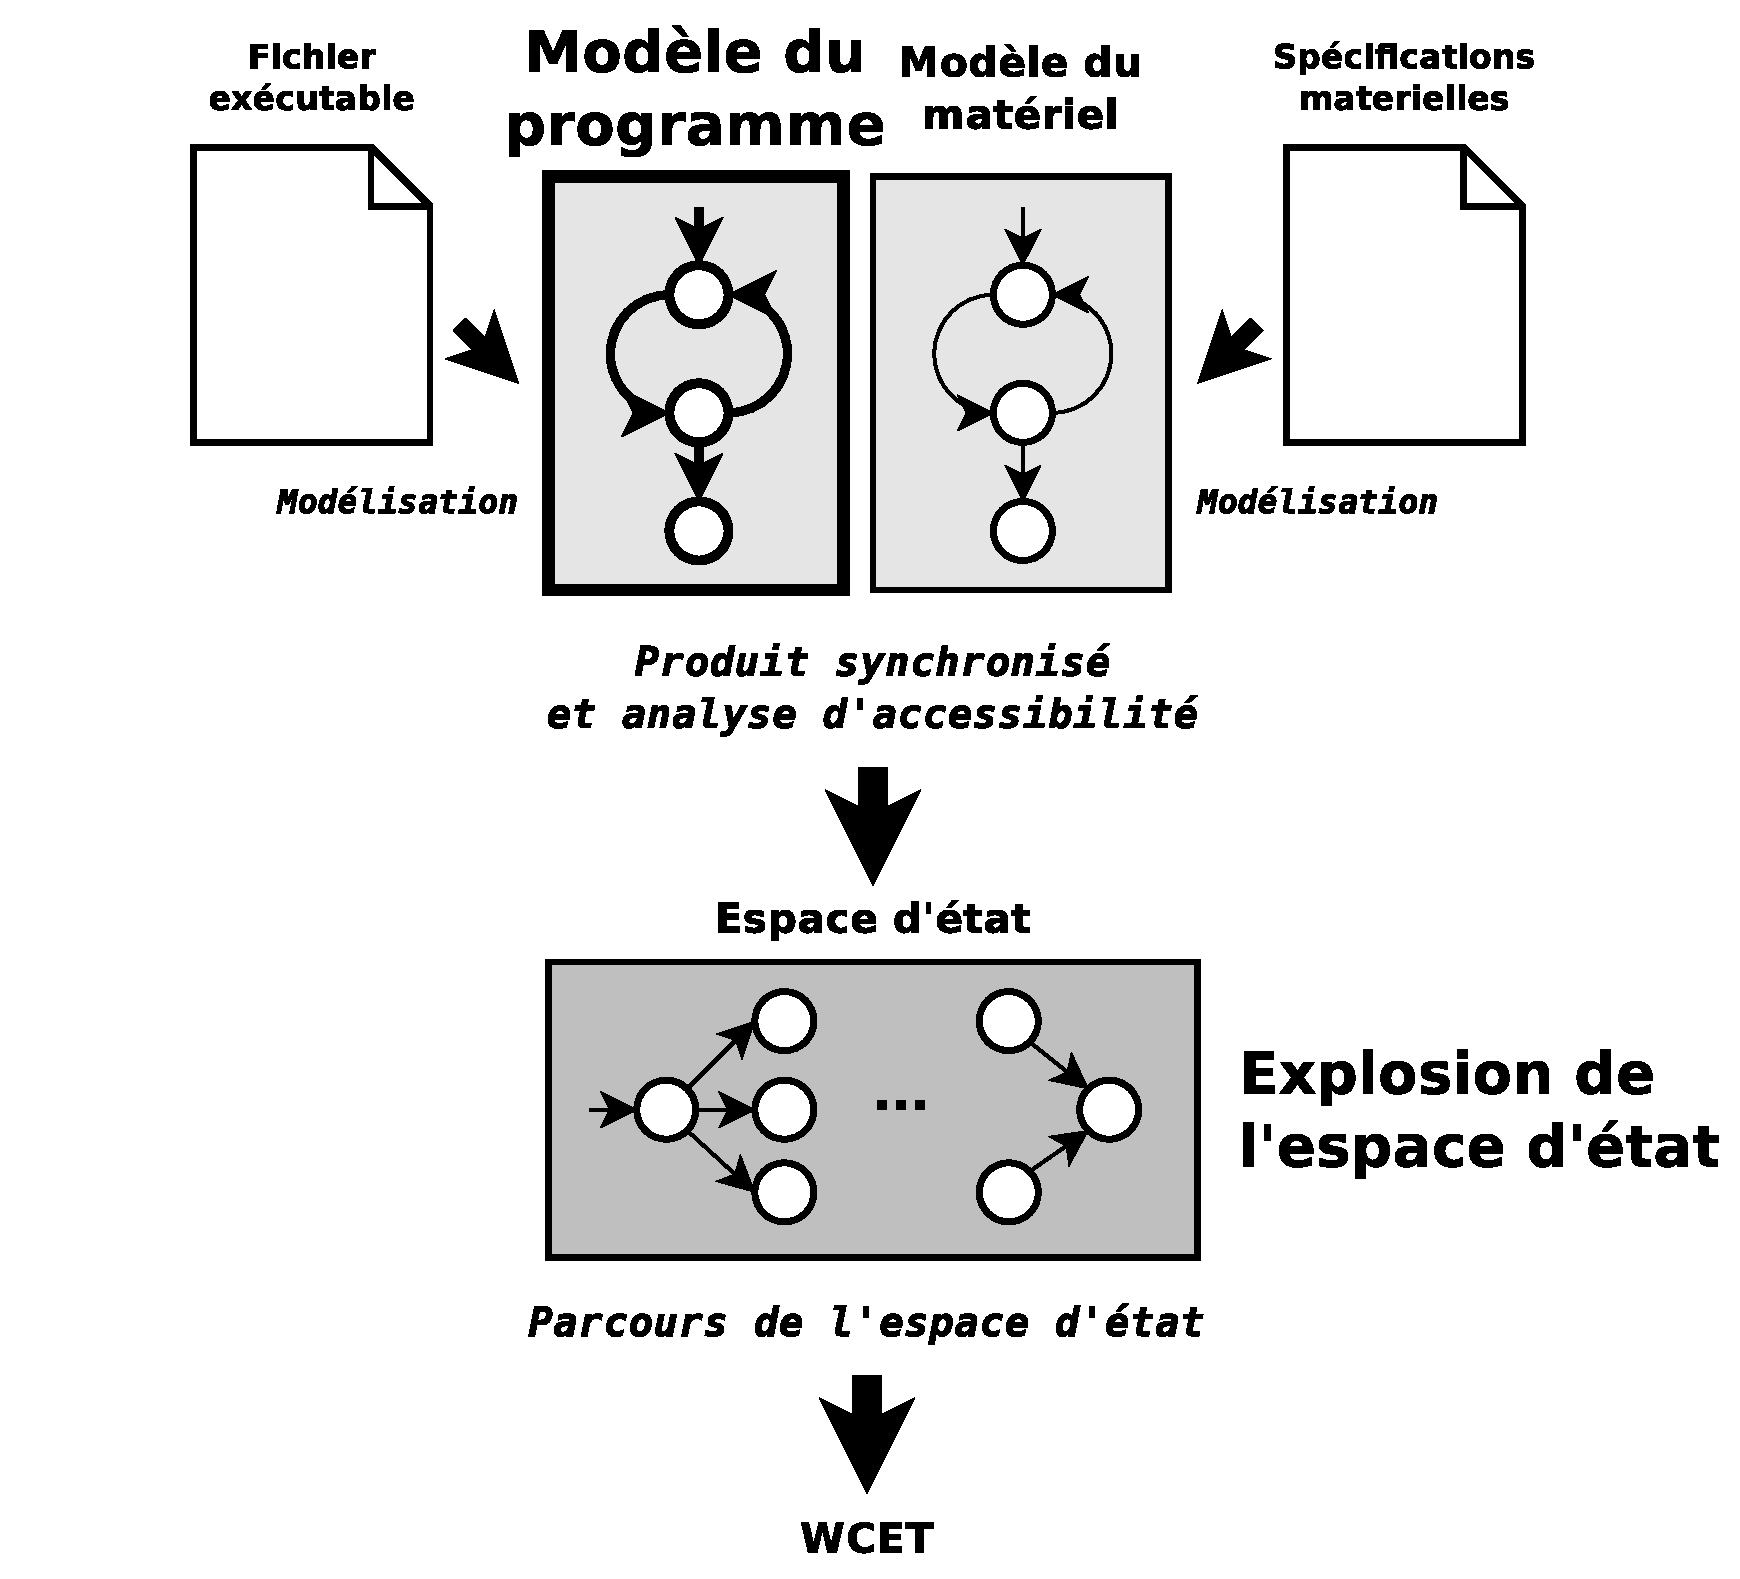
\includegraphics[height=.85\textheight]{fig/model-checking.eps}
    \end{figure}
  \end{frame}

  \begin{frame}
    \frametitle{\secname}
    \framesubtitle{\subsecname}
    
%    \begin{block}{Motivation:}
        \begin{description}
          \item[modularity] network of timed automata
          \item[tightness] exact cache analysis
            \begin{itemize} % infeasible with AI
              \item arbitrary policies (not only LRU nor PLRU)
            \end{itemize}

          \vspace{1em}
          \item[witness] initial hardware and software configuration
          \item[binary level] no high level source code analysis
            \begin{itemize}
              \item compiler independent
              %\item no problem induced by optimization options
            \end{itemize}            
        \end{description}
%    \end{block}
  \end{frame}
  
  \subsection{Challenge}
  \begin{frame}
    \frametitle{\secname}
    \framesubtitle{\subsecname}
      
    \begin{block}{Limitations}
      \begin{itemize}
      \item suffer of the state space explosion
        \begin{itemize}
        \item tailored for embedded microcontrollers % but thus precise
          \end{itemize}
      \end{itemize}
    \end{block}
    
    \vspace{1em}
    \begin{block}{Challenges}
      \begin{itemize}
        \item abstracting models of hardware components~\cite{CGM15}
        \item \textbf{abstracting models of programs}~\cite{BJ14,CB13,MBB16}
          \begin{itemize}
            \item Cassez et al., 2013
          \end{itemize}
      \end{itemize}
    \end{block}
  \end{frame}

  %%%

  \section{Program Abstraction using Program Slicing}
  \begin{frame}
    \frametitle{\secname}
    \tableofcontents[currentsection]
  \end{frame}

  \subsection{Overview of Program Slicing}
  \begin{frame}
    \frametitle{\secname}
    \framesubtitle{\subsecname}

    Introduced by Weiser in 1981~\cite{Wei81}
    \begin{itemize}
      \item given a \emph{program} $P \subseteq L \times I$, $\forall (l,i), (l,i') \in P, i = i'$ with
        \begin{itemize}
          \item $L$ a finite set of labels
          \item $I$ a finite set of instructions operating over $V$
          \item $V$ the set of variables of $P$
        \end{itemize}

      \vspace{1em}
      \item and a \emph{criterion} $C = (l,v)$ with
        \begin{itemize}
          \item $l \in L$ a label and
          \item $v \subseteq V$ a subset of variables
        \end{itemize}
        
      \vspace{1em}
      \item a \emph{slice} $S_C$ is a subset of $P$ \\
      with the same semantics as $P$ wrt. criterion $C$
    \end{itemize}
  \end{frame}

  \begin{frame}
    \frametitle{\secname}
    \framesubtitle{\subsecname}

    %\small
    The slice $S_{(l,v)}$
    \begin{itemize}
      \item is a valid program
      \item that computes values for the subset $v$
        \begin{itemize}
          \item same as with the original program $P$
          \item to the point of execution $l$ 
        \end{itemize}
      \item is obtained by deleting zero or more ``lines'' from $P$
    \end{itemize}

  \end{frame}
  
  \begin{frame}
    \frametitle{\secname}
    \framesubtitle{\subsecname}

    \vspace{1em}
    \begin{figure}
      \centering
      \begin{overlayarea}{\textwidth}{\textheight}
        \only<1>{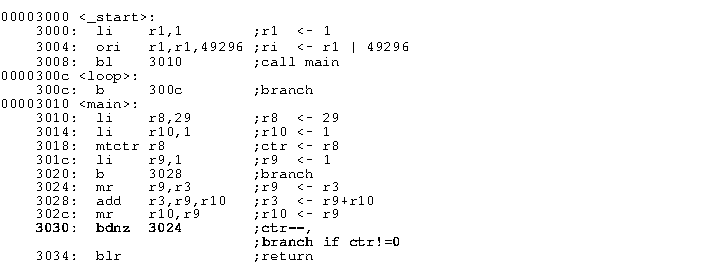
\includegraphics[scale=1.4]{fig/fibcallO2-01.pdf}}
        \only<2>{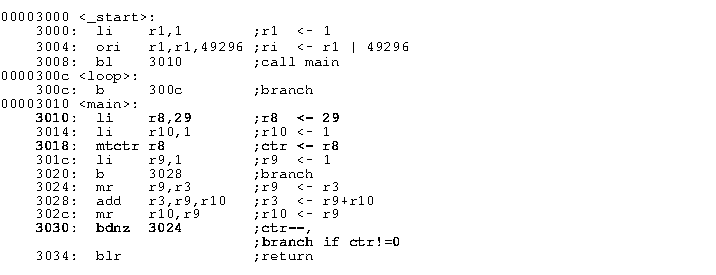
\includegraphics[scale=1.4]{fig/fibcallO2-02.pdf}}
        \begin{center}
          $C = ( 3030, \{ctr\} )$
        \end{center}
      \end{overlayarea}
    \end{figure}
  \end{frame}
  
  \begin{frame}
    \frametitle{\secname}
    \framesubtitle{\subsecname}
    
    \begin{itemize}
      \item dataflow equation-based or graph-based
        \begin{itemize}
          \item fixpoint computation or
          \item reachability analysis
        \end{itemize}
        
      \vspace{1em}
      \item slicing binary executables
      \begin{itemize}
        \item a closed issue~\cite{KJL03} (although not trivial)
        \item multiple graph computation from a CFG
        \item reachability analysis on the final graph
      \end{itemize}
      
      %% \vspace{1em}
      %% \item intuition
      %% \begin{itemize}
      %%   \item the Control Flow Graph
      %%   \item a Control Dependence Graph (of basic blocks)
      %%   \item a Data Dependence Graph (of instructions)
      %%   \item a summary Program Dependence Graph
      %% \end{itemize}
    \end{itemize}
  \end{frame}
  

  \subsection{Abstracting models of programs}
  \begin{frame}
    \frametitle{\secname}
    \framesubtitle{\subsecname}

    An instruction has
    \begin{itemize}
    \item a timing behavior due to its
      \begin{itemize}
        \item class of instruction $\rightarrow$ number of execution cycles
        \item data dependencies $\rightarrow$ pipeline stall
        \item memory access $\rightarrow$ cache delay
      \end{itemize}
      \item and a semantics
        \begin{itemize}
          \item updates the system state
        \end{itemize}
    \end{itemize}

    \begin{center}
      $\rightarrow$ We can abstract semantics of some instructions while keeping the timing behavior of the program \\
      \vspace{1em}
      $\rightarrow$ Variables used only by abstracted instructions can be removed from the model
      thus reducing the overall state space
    \end{center}

  \end{frame}

  \begin{frame}
    \frametitle{\secname}
    \framesubtitle{\subsecname}

    \begin{center}
      How to abstract a model of program? \\
      (\textbf{but not its timing behavior})
    \end{center}
    
    %\vspace{1em}
    \begin{itemize}
      \item abstract model must contain all paths from original model
        \begin{itemize}
          \item i.e. contain all control instructions and their dependencies
        \end{itemize}
        
      \vspace{1em}
      \item we can use program slicing to find these instructions
        \begin{itemize}
          \item criteria are chosen wrt. the previous constraint as follows: \\
 
          %\vspace{1em}
          $\{(l,v)~|~\exists i, ~(l,i) \in P$ \\
          \hspace{5em} and $i$ is a conditional branching instruction \\
          \hspace{5em} and $v$ is the subset of variables used by $i$ at $l \}$
        \end{itemize}
      %\vspace{1em}
      %  $\rightarrow$ a criterion $(l,v)$ with $v$ being used by $i$
    \end{itemize}
  \end{frame}

  \begin{frame}
    \frametitle{\secname}
    \framesubtitle{\subsecname}

    % TODO: How to choose the criterion: What are the "useless" instructions?
    \begin{figure}
      \centering
      \only<1>{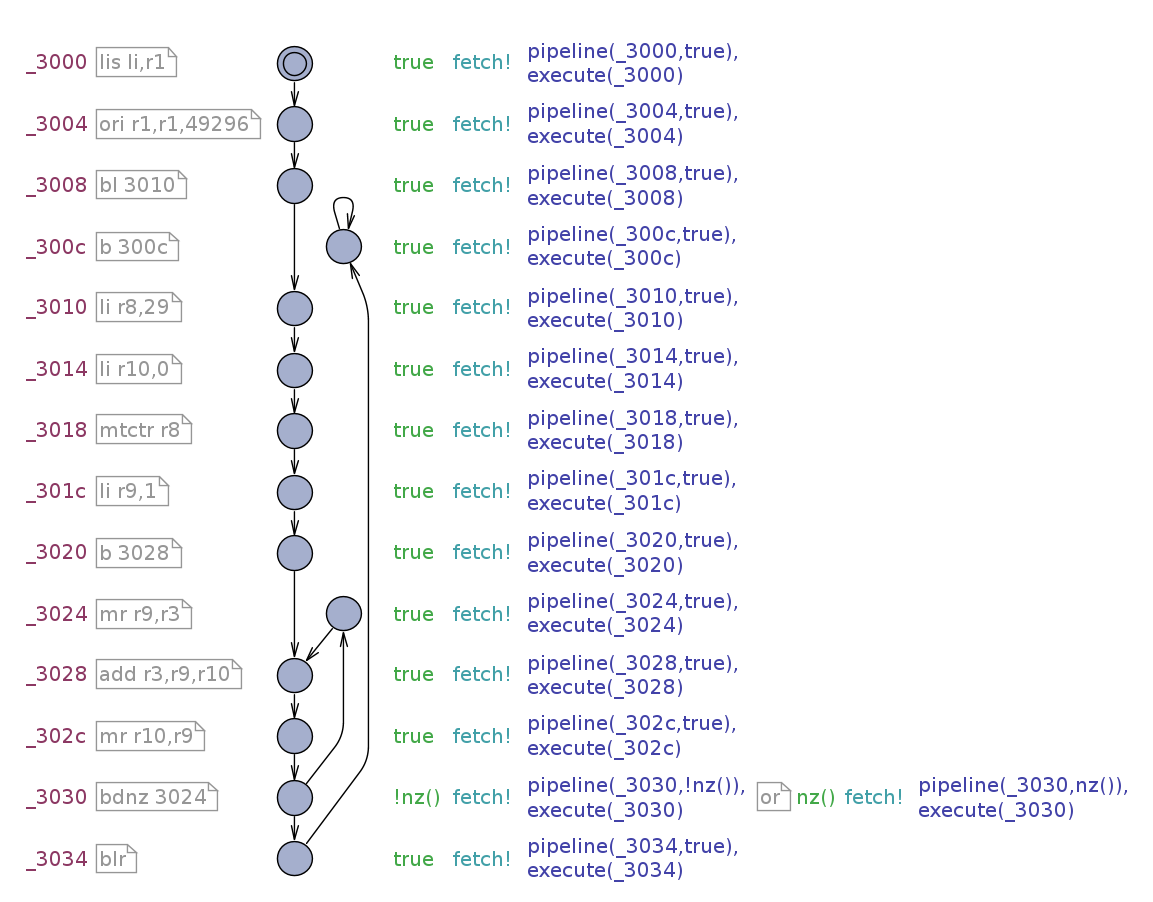
\includegraphics[height=.85\textheight]{fig/example0.png}} % TODO
      \only<2>{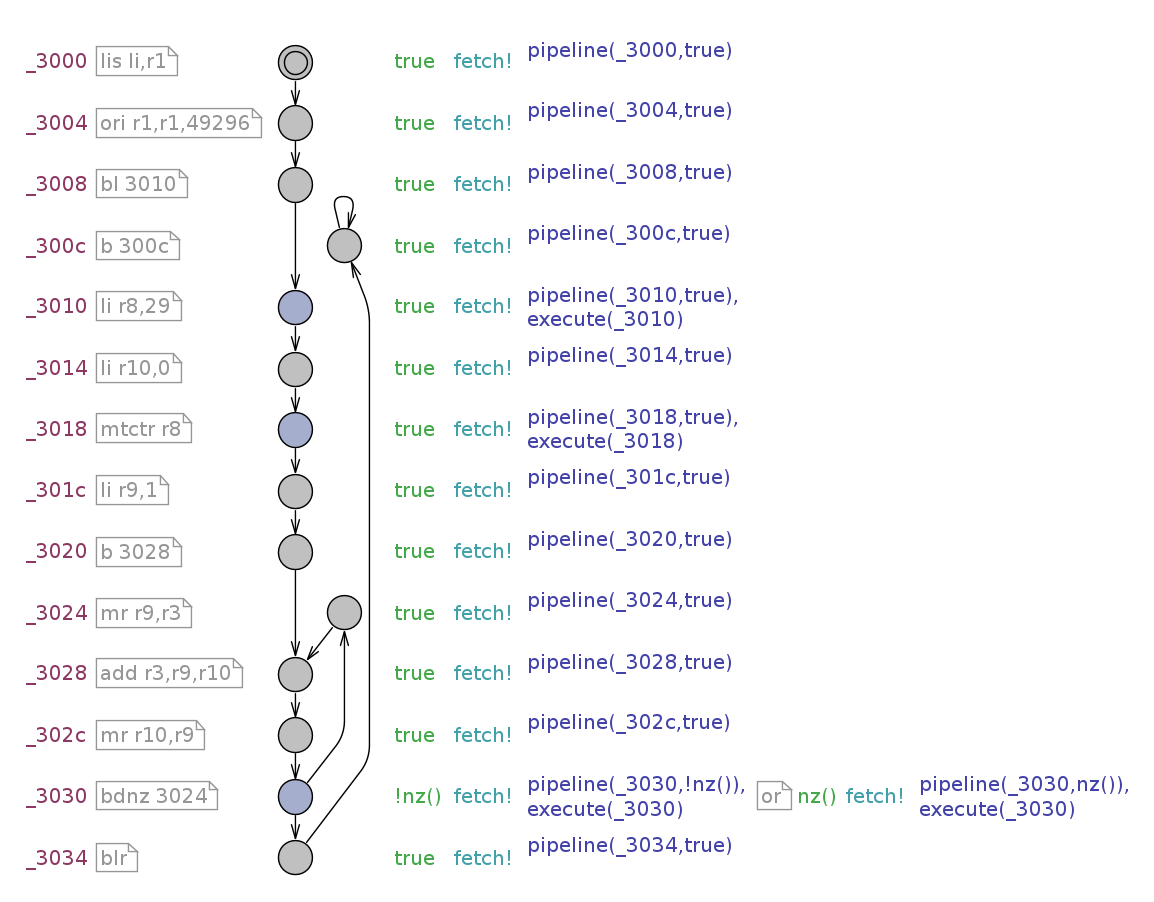
\includegraphics[height=.85\textheight]{fig/example1.png}}
    \end{figure}

    %% \begin{itemize}
    %%   \item how to abstract models of program using program slicing?
    %%   \item removing instructions would results in losing essential information
    %%     regarding registers use and thus pipeline timing behavior.
    %%   \item so we can't remove instructions

    %%   \item what can we remove?
        
    %%   \item How do we use Program Slicing to abstract models of programs?
      
    %%   \vspace{1em}
    %%   \item Abstracted models of programs keep the same time behaviour as
    %%     unabstracted models.
    %%   \item We do not intend to perform WCET analysis on slices but on abstracts
    %%     models of programs built using information gathered through program
    %%     slicing.
    %%   \item Instructions not in the slice are abstracted (not removed, they keep
    %%     their time behaviour) others are not.
    %% \end{itemize}
  \end{frame}
  
  \subsection{Tool implementation}
  \begin{frame}
    \frametitle{\secname}
    \framesubtitle{\subsecname}

    \begin{figure}
      \centering
      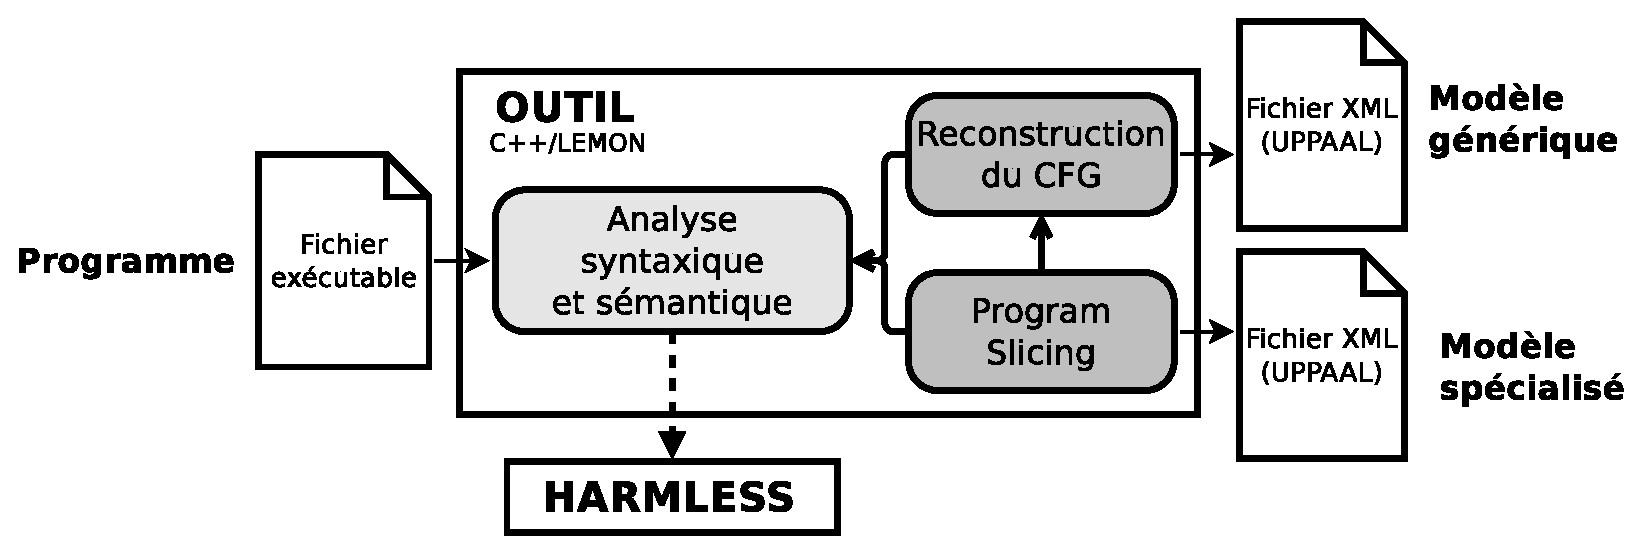
\includegraphics[height=.7\textheight]{fig/archi.eps}
    \end{figure}
  \end{frame}

  %%%
  
  \section{Experimental results}
  \begin{frame}
    \frametitle{\secname}
    \tableofcontents[currentsection]
  \end{frame}
  
  \subsection{Methodology}
  \begin{frame}
    \frametitle{\secname}
    \framesubtitle{\subsecname}

    \begin{itemize}
      \item use of Mälardalen WCET benchmarks
      \item excluding programs containing % 16 out of the 35
        \begin{itemize}
          \item switch-case statements % whereas it's a closed issue
          \item floating-point arithmetic % missing in the PowerPC HADL file 
          \item recursive programs
        \end{itemize}
      \item multiple compilers and optimization options
        \begin{itemize}
          \item \textsc{Gcc} 5.3.1 (\texttt{-O0}, \texttt{-O1}, \texttt{-O2}, \texttt{-O3})
          \item \textsc{Cosmic C} 4.3.7 (\texttt{-no}, \emph{default})
          \item targeting the PowerPC 32 bits instruction set
        \end{itemize}
      \item sums up to 96 binaries

      \vspace{1em}
      \item use of Trampoline RTOS~\cite{BBF06} services
        \begin{itemize}
          \item not documented on our paper
        \end{itemize}
    \end{itemize}
  \end{frame}
  
  \subsection{Results}
  \begin{frame}
    \frametitle{\secname}
    \framesubtitle{\subsecname}

    \begin{table}
      \centering
      \begin{overlayarea}{\textwidth}{.2\textheight}
        \only<1>{
          \scalebox{.55}{\begin{tabular}{ |l| |c|c|c|c| |c|c| }
  \hline
  \multirow{2}{*}{Source file}
  & \multicolumn{4}{c||}{\textsc{Gcc}}
  & \multicolumn{2}{c|}{\textsc{Cosmic C}}

  \\\cline{2-7}
  & \multicolumn{1}{c|}{\texttt{-O0}} & \multicolumn{1}{c|}{\texttt{-O1}} & \multicolumn{1}{c|}{\texttt{-O2}} & \multicolumn{1}{c||}{\texttt{-O3}}
  & \multicolumn{1}{c|}{\texttt{-no}} & \multicolumn{1}{c|}{\emph{default}}

  \\\hline\hline
  \verb|adpcm.c|
  & $224/1858$, $88\%$ & $357/966$, $63\%$ & $421/1094$, $62\%$ & $348/1775$, $80\%$
&               $398/1282$,                $69\%$ &               $338/1064$,                $68\%$

    \\\hline\hline
  \multirow{2}{*}{Average}
  & \multicolumn{1}{c|}{$78\%$} & \multicolumn{1}{c|}{$63\%$} & \multicolumn{1}{c|}{$62\%$} & \multicolumn{1}{c||}{$65\%$}
  & \multicolumn{1}{c|}{$66\%$} & \multicolumn{1}{c|}{$63\%$}

  \\\cline{2-7}  
  & \multicolumn{4}{c||}{$67\%$}
  & \multicolumn{2}{c|}{$64\%$}

  \\\hline
\end{tabular}
}\hfill\\\vspace{1em}
          \scriptsize $\rightarrow$ number of instructions in the slice/total number of
          instructions, gain in percentage.\\
          \scriptsize $\rightarrow$ execution time negligible (always < 1 sec.)}
          %\scalebox{.8}{\begin{tabular}{|c|c| |c|c|c|c|}
   \hline
   \multirow{2}{*}{Compiler} & \multirow{2}*{Optim.} & \multicolumn{4}{c|}{Instructions in slice} 
   \\\cline{3-6}
    & & Avg. & Min & Max. & Std. dev. 

    \\\hline\hline
    \multirow{4}{*}{\textsc{Gcc}} & \verb|-O0| & 21.6\% & 1.7\% & 43.2\% & 8.9\%
    
    \\\cline{2-6}
     & \verb|-O1| & 36.7\% & 3.24\% & 67.9\% & 10.2\%
    
    \\\cline{2-6}
     & \verb|-O2| & 37.8\% & 2.9\% & 72.5\% & 15.7\%
    
    \\\cline{2-6}
     & \verb|-O3| & 34.7\% & 0.4\% & 72.2\% & 18\%


     \\\hline\hline
     \multirow{2}*{\textsc{Cosmic C}} & \verb|-no| & 34\% & 1.9\% & 60.2\% & 15.2\% 
    
     \\\cline{2-6}
     & \emph{default} & 37\% & 2.8\% & 66.7\% & 15.8\% 
  
     \\\hline
\end{tabular}

}\hfill\\\vspace{1em}
          %\scriptsize $\rightarrow$ gains in percentage.}
        \only<2>{
          \scalebox{.55}{\begin{tabular}{ |l| |c|c|c|c| |c|c| }
  \hline
  \multirow{2}{*}{Source file}
  & \multicolumn{4}{c||}{\textsc{Gcc}}
  & \multicolumn{2}{c|}{\textsc{Cosmic C}}

  \\\cline{2-7}
  & \multicolumn{1}{c|}{\texttt{-O0}} & \multicolumn{1}{c|}{\texttt{-O1}} & \multicolumn{1}{c|}{\texttt{-O2}} & \multicolumn{1}{c||}{\texttt{-O3}}
  & \multicolumn{1}{c|}{\texttt{-no}} & \multicolumn{1}{c|}{\emph{default}}

  \\\hline\hline
  \verb|adpcm.c|
  & $11/17$, $35\%$ & $28/32$, $13\%$ & $26/28$, $7\%$ & $33/36$, $8\%$
  & $22/37$, $41\%$ & $22/37$, $41\%$

    \\\hline\hline
  \multirow{2}{*}{Average}
  & \multicolumn{1}{c|}{$38\%$} & \multicolumn{1}{c|}{$35\%$} & \multicolumn{1}{c|}{$36\%$} & \multicolumn{1}{c||}{$37\%$}
  & \multicolumn{1}{c|}{$59\%$} & \multicolumn{1}{c|}{$54\%$}

  \\\cline{2-7}  
  & \multicolumn{4}{c||}{$37\%$}
  & \multicolumn{2}{c|}{$57\%$}

  \\\hline
\end{tabular}
}\hfill\\\vspace{1em}
          \scriptsize $\rightarrow$ number of registers in the slice/total number of
          registers, gain in percentage.\\
          \scriptsize $\rightarrow$ execution time negligible (always < 1 sec.)}
          %\scalebox{.8}{\begin{tabular}{|c|c| |c|c|c|c|}
   \hline
   \multirow{2}{*}{Compiler} & \multirow{2}*{Optim.} & \multicolumn{4}{c|}{Registers in slice}
   \\\cline{3-6}
    & &  Avg. & Min & Max. & Std. dev.

    \\\hline\hline
    \multirow{4}{*}{\textsc{Gcc}} & \verb|-O0| & 61.8\% & 43.7\%  & 78.9\% & 8.8\%
    
    \\\cline{2-6}
     & \verb|-O1| & 64.6\% & 19.1\%  & 87.5\% & 13.6\%
    
    \\\cline{2-6}
     & \verb|-O2| & 64.3\% & 13.3\%  & 92.9\% & 20.3\%
    
    \\\cline{2-6}
     & \verb|-O3| & 62.8\% & 9\%  & 96.4\% & 21.7\%


     \\\hline\hline
     \multirow{2}*{\textsc{Cosmic C}} & \verb|-no| & 40.5\% & 8.6\% & 86.7\% & 16.6\%
    
     \\\cline{2-6}
     & \emph{default} & 37\% & 2.8\% & 66.7\% & 15.8\%
  
     \\\hline
\end{tabular}

}\hfill\\\vspace{1em}
          %\scriptsize $\rightarrow$ gains in percentage.}
      \end{overlayarea}
    \end{table}    
    
    %\vspace{1em}
    %\begin{center}
    %  \scriptsize $\rightarrow$ execution time negligible (always < 1 sec.)
    %\end{center}
  \end{frame}
  
  %%%
  
  \section{Future work}
  \begin{frame}
    \frametitle{\secname}
    \tableofcontents[currentsection]
  \end{frame}
  
  \begin{frame}
    \frametitle{\secname}

    \begin{itemize}
      %\item can not account for indirect branch
      \item improve support of interprocedurality (straightforward) % suboptimal
      \item extend data dependency analysis to stack frames and initialized data
      \begin{itemize}
        \item bigger slices but not necessarily bigger state space
      \end{itemize}

      \vspace{1em}
      \item modeling the PowerPC e200z4 core
        \begin{itemize}
          \item no data cache
          \item instruction cache
            \begin{itemize}
              \item 2 or 4-ways associative
              \item pseudorandom (global FIFO)
            \end{itemize}
          \item branch prediction, \dots
        \end{itemize}
      \item modeling the MPC5643L microcontroller
        \begin{itemize}
          \item two PowerPC e200z4 cores
          \item XBAR crossbar switch
            \begin{itemize}
              \item multiple masters / multiple slaves
              \item per slave policy (FP or RR)
            \end{itemize}
        \end{itemize}

      \vspace{1em}
      \item WCET analysis of parallel programs
    \end{itemize}
  \end{frame}

  %%%

  \section*{Conclusion}
  \begin{frame}
    \frametitle{\secname}

    \begin{itemize}
    \item abstract models of program
      \begin{itemize}
        \item for Model Checking-based WCET analysis
        \item based on program slicing
      \end{itemize}
      
    \vspace{1em}
    \item a binary executable slicing tool
      \begin{itemize}
        \item instruction set independant
        \item free sofware (GNU GPL)
        \item promising experimental results
      \end{itemize}

      %  \begin{itemize}
      %    \item instruction set independent
      %  \end{itemize}
      %\item thanks to (a re-targeting of) HARMLESS
      %  \begin{itemize}
      %    \item primarly a generator of cycle accurate simulators
      %    \item based on a hardware architecture description language (HADL)
      %  \end{itemize}

      %\vspace{1em}
      %\item free software under General Public License % free as in freedom
      %\item written in C++ and using LEMON~\cite{DJK11}
      %\item outputs textual, Graphviz and UPPAAL files
    \end{itemize}
  \end{frame}
  
  %%%
  
  \appendix
  \section{References}
  \begin{frame}%[allowframebreaks]
    \frametitle{\secname}
    \tiny
    
    \bibliographystyle{plain}
    \bibliography{src/refs.bib}
  \end{frame}

  \begin{frame}
    \frametitle{Expermimental results}
    \framesubtitle{Detailed results}

    \begin{table}
      \centering
      \scalebox{.5}{\begin{tabular}{ |l| |c|c|c|c| |c|c| }
  \hline
  \multirow{2}{*}{Source file}
  & \multicolumn{4}{c||}{\textsc{Gcc}}
  & \multicolumn{2}{c|}{\textsc{Cosmic C}}

  \\\cline{2-7}
  & \multicolumn{1}{c|}{\texttt{-O0}} & \multicolumn{1}{c|}{\texttt{-O1}} & \multicolumn{1}{c|}{\texttt{-O2}} & \multicolumn{1}{c||}{\texttt{-O3}}
  & \multicolumn{1}{c|}{\texttt{-no}} & \multicolumn{1}{c|}{\emph{default}}

  \\\hline\hline
  \verb|adpcm.c|
  & $1858/224$, $88\%$ & $966/357$, $63\%$ & $1094/421$, $62\%$ & $1775/348$, $80\%$
&               $1282/398$,                $69\%$ &               $1064/338$,                $68\%$
  
  \\\hline
  \verb|bs.c|
  & \hspace{1em}$   82/27$,\hspace{.5em}$67\%$ & \hspace{.5em}$  38/19$,\hspace{.5em}$50\%$ & \hspace{1em}$   28/18$,\hspace{.5em}$36\%$ & \hspace{1em}$   28/18$,\hspace{.5em}$36\%$
& \hspace{1em}$54/28$,    \hspace{.5em}$48\%$ & \hspace{1em}$35/18$,     \hspace{.5em}$49\%$

  \\\hline
  \verb|bsort100.c|
  & \hspace{.5em}$  141/39$,\hspace{.5em}$72\%$ & \hspace{.5em}$  65/24$,\hspace{.5em}$63\%$ & \hspace{1em}$   58/18$,\hspace{.5em}$69\%$ & \hspace{1em}$   58/18$,\hspace{.5em}$69\%$
& \hspace{1em}$74/34$,    \hspace{.5em}$54\%$ & \hspace{1em}$66/34$,     \hspace{.5em}$48\%$

  \\\hline
  \verb|cnt.c|
  & \hspace{.5em}$  193/44$,\hspace{.5em}$77\%$ & $ 104/38$,\hspace{.5em}$63\%$ & \hspace{1em}$   87/24$,\hspace{.5em}$72\%$ & $ 1124/81$,\hspace{.5em}$93\%$
& \hspace{.5em}$128/25$,    \hspace{.5em}$80\%$ & \hspace{.5em}$112/23$,    \hspace{.5em}$79\%$

  \\\hline
  \verb|compress.c|
  & \hspace{.5em}$ 725/271$, $63\%$ & $529/214$, $60\%$ & \hspace{.5em}$ 530/247$, $53\%$ & \hspace{.5em}$ 752/316$, $58\%$
& \hspace{.5em}$591/253$,                 $57\%$ & \hspace{.5em}$501/228$,                 $54\%$

  \\\hline
  \verb|crc.c|
  & \hspace{.5em}$  295/44$,\hspace{.5em}$85\%$ & $ 162/50$,\hspace{.5em}$69\%$ & \hspace{.5em}$  141/47$,\hspace{.5em}$67\%$ & \hspace{.5em}$  210/98$,\hspace{.5em}$53\%$
& \hspace{.5em}$186/112$,                 $40\%$ & \hspace{.5em}$148/81$,    \hspace{.5em}$45\%$

  \\\hline
  \verb|expint.c|
  & \hspace{.5em}$  187/33$,\hspace{.5em}$82\%$ & $ 135/50$,\hspace{.5em}$63\%$ & \hspace{1em}$    27/5$,\hspace{1em}$81\%$ & \hspace{1em}$    27/5$,\hspace{1em}$81\%$
& \hspace{.5em}$115/48$,    \hspace{.5em}$58\%$ & \hspace{1em}$93/40$,     \hspace{.5em}$57\%$

  \\\hline
  \verb|fdct.c|
  & \hspace{.5em}$  662/11$,\hspace{.5em}$98\%$ & $  185/6$,\hspace{1em}$97\%$ & \hspace{.5em}$   205/6$,\hspace{1em}$97\%$ & \hspace{.5em}$   692/3$,\hspace{1em}$99\%$
& \hspace{.5em}$317/6$,     \hspace{1em}$98\%$ & \hspace{.5em}$218/6$,     \hspace{1em}$97\%$

  \\\hline
  \verb|fibcall.c|
  & \hspace{1em}$   58/12$,\hspace{.5em}$79\%$ & \hspace{.5em}$  32/10$,\hspace{.5em}$69\%$ & \hspace{1em}$    14/3$,\hspace{1em}$79\%$ & \hspace{1em}$    14/3$,\hspace{1em}$79\%$
& \hspace{1em}$29/8$,      \hspace{1em}$72\%$ & \hspace{1em}$21/8$,      \hspace{1em}$62\%$

  \\\hline
  \verb|fir.c|
  & \hspace{.5em}$  137/21$,\hspace{.5em}$85\%$ & \hspace{.5em}$  79/34$,\hspace{.5em}$57\%$ & \hspace{1em}$   79/33$,\hspace{.5em}$58\%$ & \hspace{1em}$   79/33$,\hspace{.5em}$58\%$
& \hspace{1em}$87/35$,     \hspace{.5em}$60\%$ & \hspace{1em}$74/30$,     \hspace{.5em}$59\%$

  \\\hline
  \verb|janne_complex.c|
  & \hspace{1em}$   75/21$,\hspace{.5em}$72\%$ & \hspace{.5em}$  39/21$,\hspace{.5em}$46\%$ & \hspace{1em}$   40/29$,\hspace{.5em}$28\%$ & \hspace{1em}$   36/26$,\hspace{.5em}$28\%$
& \hspace{1em}$41/20$,     \hspace{.5em}$51\%$ & \hspace{1em}$30/20$,     \hspace{.5em}$33\%$

  \\\hline
  \verb|jfdctint.c|
  & \hspace{.5em}$  505/29$,\hspace{.5em}$94\%$ & $  195/9$,\hspace{1em}$95\%$ & \hspace{.5em}$   219/9$,\hspace{1em}$96\%$ & \hspace{.5em}$   795/6$,\hspace{1em}$99\%$
& \hspace{.5em}$255/9$,     \hspace{1em}$96\%$ & \hspace{.5em}$205/9$,     \hspace{1em}$96\%$

  \\\hline
  \verb|matmult.c|
  & \hspace{.5em}$  196/36$,\hspace{.5em}$82\%$ & $ 120/42$,\hspace{.5em}$65\%$ & \hspace{.5em}$  110/43$,\hspace{.5em}$61\%$ & \hspace{.5em}$  103/38$,\hspace{.5em}$63\%$
& \hspace{.5em}$135/20$,    \hspace{.5em}$85\%$ & \hspace{.5em}$118/20$,    \hspace{.5em}$83\%$

  \\\hline
  \verb|ndes.c|
  & \hspace{.5em}$ 936/162$, $83\%$ & $474/160$, $66\%$ & \hspace{.5em}$ 563/236$, $58\%$ & \hspace{.5em}$ 886/522$, $41\%$
& \hspace{.5em}$653/118$,                 $82\%$ & \hspace{.5em}$576/112$,                 $81\%$

  \\\hline
  \verb|ns.c|
  & \hspace{.5em}$  115/35$,\hspace{.5em}$66\%$ & \hspace{.5em}$  65/30$,\hspace{.5em}$54\%$ & \hspace{1em}$   46/27$,\hspace{.5em}$41\%$ & \hspace{.5em}$  181/88$,\hspace{.5em}$51\%$
& \hspace{1em}$69/33$,     \hspace{.5em}$52\%$ & \hspace{1em}$54/29$,     \hspace{.5em}$46\%$

  \\\hline
  \verb|prime.c|
  & \hspace{.5em}$  146/63$,\hspace{.5em}$57\%$ & \hspace{.5em}$  56/38$,\hspace{.5em}$32\%$ & \hspace{1em}$   48/30$,\hspace{.5em}$38\%$ & \hspace{1em}$   31/14$,\hspace{.5em}$55\%$
& \hspace{1em}$95/46$,     \hspace{.5em}$52\%$ & \hspace{1em}$82/42$,     \hspace{.5em}$49\%$

  \\\hline\hline
  \multirow{2}{*}{Average}
  & \multicolumn{1}{c|}{$78\%$} & \multicolumn{1}{c|}{$63\%$} & \multicolumn{1}{c|}{$62\%$} & \multicolumn{1}{c||}{$65\%$}
  & \multicolumn{1}{c|}{$66\%$} & \multicolumn{1}{c|}{$63\%$}

  \\\cline{2-7}  
  & \multicolumn{4}{c||}{$67\%$}
  & \multicolumn{2}{c|}{$64\%$}
  
  \\\hline
\end{tabular}
}
    \end{table}
    
    \vspace{-1em}
    \begin{center}
      \scriptsize $\rightarrow$ number of instructions in the slice / total number of
      instructions, \\ gain in percentage.
    \end{center}
  \end{frame}

  \begin{frame}
    \frametitle{Expermimental results}
    \framesubtitle{Detailed results}

    \begin{table}
      \centering
      \scalebox{.5}{\begin{tabular}{ |l| |c|c|c|c| |c|c| }
  \hline
  \multirow{2}{*}{Source file}
  & \multicolumn{4}{c||}{\textsc{Gcc}}
  & \multicolumn{2}{c|}{\textsc{Cosmic C}}

  \\\cline{2-7}
  & \multicolumn{1}{c|}{\texttt{-O0}} & \multicolumn{1}{c|}{\texttt{-O1}} & \multicolumn{1}{c|}{\texttt{-O2}} & \multicolumn{1}{c||}{\texttt{-O3}}
  & \multicolumn{1}{c|}{\texttt{-no}} & \multicolumn{1}{c|}{\emph{default}}

  \\\hline\hline
  \verb|adpcm.c|
  & $11/17$, $35\%$ & $28/32$, $13\%$ & $26/28$,\hspace{.5em} $7\%$ & $33/36$,\hspace{.5em} $8\%$
  & $22/37$, $41\%$ & $22/37$, $41\%$
  
  \\\hline
  \verb|bs.c|
  & $7/11$, $36\%$ & $10/13$, $23\%$ & $9/10$, $10\%$ & $9/10$, $10\%$
  & $10/14$, $29\%$ & $11/13$, $15\%$
  
  \\\hline
  \verb|bsort100.c|
  & $9/12$, $25\%$ & $13/18$, $28\%$ & $11/16$, $31\%$ & $11/16$, $31\%$
  & $13/15$, $13\%$ & $13/15$, $13\%$

  \\\hline
  \verb|cnt.c|
  & $10/15$, $33\%$ & $13/18$, $28\%$ & $10/16$, $38\%$ & $10/18$, $44\%$
  & $10/37$, $73\%$ & $10/37$, $73\%$

  \\\hline
  \verb|compress.c|
  & $15/19$, $21\%$ & $26/31$, $16\%$ & $30/33$,\hspace{.5em} $9\%$ & $32/35$,\hspace{.5em} $9\%$
  & $21/37$, $43\%$ & $21/37$, $43\%$

  \\\hline
  \verb|crc.c|
  & $8/17$, $53\%$ & $14/23$, $39\%$ & $10/19$, $47\%$ & $9/19$, $53\%$
  & $18/37$, $51\%$ & $18/37$, $51\%$

  \\\hline
  \verb|expint.c|
  & $8/13$, $38\%$ & $16/26$, $38\%$ & $4/11$, $64\%$ & $4/11$, $63\%$
  & $14/37$, $62\%$ & $14/37$, $62\%$

  \\\hline
  \verb|fdct.c|
  & $6/13$, $54\%$ & $4/21$, $81\%$ & $4/30$, $87\%$ & $3/33$, $91\%$
  & $3/35$, $91\%$ & $3/35$, $91\%$

  \\\hline
  \verb|fibcall.c|
  & $7/11$, $36\%$ & $7/12$, $42\%$ & $3/7$,\hspace{.5em} $57\%$ & $3/7$,\hspace{.5em} $57\%$
  & $6/12$, $50\%$ & $6/10$, $40\%$

  \\\hline
  \verb|fir.c|
  & $7/16$, $56\%$ & $13/22$, $41\%$ & $14/21$, $33\%$  & $14/21$, $33\%$
  & $15/37$, $59\%$ & $15/37$, $59\%$

  \\\hline
  \verb|janne_complex.c|
  & $7/12$, $42\%$ & $6/9$,\hspace{.5em} $33\%$ & $6/8$,\hspace{.5em} $25\%$ & $7/9$,\hspace{.5em} $22\%$
  & $7/36$, $81\%$ & $7/8$,\hspace{.5em} $13\%$

  \\\hline
  \verb|jfdctint.c|
  & $8/11$, $27\%$ & $3/15$, $80\%$ & $4/25$, $84\%$ & $4/33$, $88\%$
  & $3/35$, $91\%$ & $3/34$, $91\%$
  
  \\\hline
  \verb|matmult.c|
  & $10/19$, $47\%$ & $15/20$, $25\%$ & $15/19$, $21\%$ & $13/19$, $32\%$
  & $8/37$, $78\%$ & $8/37$, $78\%$

  \\\hline
  \verb|ndes.c|
  & $9/17$, $47\%$ & $21/27$, $22\%$  & $23/26$, $12\%$ & $27/28$,\hspace{.5em} $4\%$
  & $16/37$, $57\%$ & $15/37$, $59\%$

  \\\hline
  \verb|ns.c|
  & $9/14$, $36\%$ & $13/17$, $24\%$ & $13/15$, $13\%$ & $9/12$, $25\%$ 
  & $14/37$, $62\%$ & $14/36$, $61\%$

  \\\hline
  \verb|prime.c|
  & $10/13$, $23\%$ & $6/9$,\hspace{.5em} $33\%$ & $6/9$,\hspace{.5em} $33\%$ & $6/8$,\hspace{.5em} $25\%$
  & $11/36$, $69\%$ & $12/36$, $67\%$

  \\\hline\hline
  \multirow{2}{*}{Average}
  & \multicolumn{1}{c|}{$38\%$} & \multicolumn{1}{c|}{$35\%$} & \multicolumn{1}{c|}{$36\%$} & \multicolumn{1}{c||}{$37\%$}
  & \multicolumn{1}{c|}{$59\%$} & \multicolumn{1}{c|}{$54\%$}

  \\\cline{2-7}  
  & \multicolumn{4}{c||}{$37\%$}
  & \multicolumn{2}{c|}{$57\%$}
    
  \\\hline
\end{tabular}
}
    \end{table}

    \vspace{-1em}
    \begin{center}
      \scriptsize $\rightarrow$ number of memory locations in the slice / total number of
      memory locations, \\ gain in percentage.
    \end{center}
  \end{frame}

  
\end{document}
